\lab{Newton and Quasi-Newton Methods}{Newton and Quasi-Newton Methods}

\objective{Newton's method is the basis of several iterative methods for optimization.
Though it converges quickly, it is often very computationally expensive.
Variants on Newton's method, including BFGS, remedy the problem somewhat by numerically approximating Hessian matrices.
In this lab we implement Newton's method, BFGS, and the Gauss-Newton method for nonlinear least squares problems.}

% Newton's method is generally useful because of its fast convergence properties.
% However, Newton's method requires the explicit calculation of the second derivative (i.e., the Hessian matrix) at each step, which is computationally costly.
% Quasi-Newton methods modify Newton's method so that the Hessian does not have to be computed at each step, thus making computations faster.
% This generally comes at the cost of slower convergence speed, but the increased computation speed can make these methods more effective in many cases.

\section*{Newton's Method} % ==================================================

For $g:\mathbb{R}\rightarrow\mathbb{R}$, Newton's method finds a root $\bar{x}$ of the equation $g(x) = 0$ with the following rule.
\begin{equation}
x_{k+1} = x_{k} - \frac{g(x_k)}{g'(x_k)}
\label{eq:quasinewton-newton1d-root}
\end{equation}
Let $f:\mathbb{R}\rightarrow\mathbb{R}$.
Substituting $g = f'$ into \eqref{eq:quasinewton-newton1d-root} yields an iterative method for locating a critical point $x^*$ of $f$ satisfying $f'(x^*) = 0$.
\begin{equation}
x_{k+1} = x_{k} - \frac{f'(x_k)}{f''(x_k)}
\label{eq:quasinewton-newton1d}
\end{equation}

This technique generalizes to higher dimensions.
For $g:\mathbb{R}^n \rightarrow \mathbb{R}^n$, the following iterative technique finds $\bar{\x}$ such that $g(\bar{\x}) = \0$.
\begin{equation}
\x_{k+1} = \x_k - Dg(\x_k)^{-1}g(\x_k)
\label{eq:quasinewton-newtonroot-nd}
\end{equation}
Now let $f:\mathbb{R}^n\rightarrow\mathbb{R}$.
To calculate an optimal value $\x^*$ of $f$ satisfying $Df(\x^*) = \0$, plug $g = Df$ into \eqref{eq:quasinewton-newtonroot-nd} to get the following equation.
\begin{equation}
\x_{k+1} = \x_k - D^2f(\x_k)^{-1}Df(\x_k)\trp
\label{eq:quasinewton-newton-nd}
\end{equation}
Here the first derivative $Df:\mathbb{R}^n\rightarrow\mathbb{R}^n$ evaluates to the row vector $Df(\x) = [D_{1}f(\x)\ \ldots\ D_{n}f(\x)]$,
and the second derivative $D^2f:\mathbb{R}^n\rightarrow\mathbb{R}^{n\times n}$ evaluates to the $n\times n$ \emph{Hessian} matrix
\[
D^2f(\x) =
\left[\begin{array}{ccc}
D_1 D_1 f(\x) & \ldots & D_n D_1 f(\x) \\
D_1 D_2 f(\x) & \ldots & D_n D_2 f(\x) \\
\vdots        &        & \vdots        \\
D_1 D_n f(\x) & \ldots & D_n D_n f(\x)
\end{array}\right]
=
\left[\begin{array}{ccc}
\frac{\partial^2 f}{\partial x_1 \partial x_1} & \cdots & \frac{\partial^2 f}{\partial x_n \partial x_1} \\
\vdots & \ddots & \vdots \\
\frac{\partial^2 f}{\partial x_1 \partial x_n} & \cdots & \frac{\partial^2 f}{\partial x_n \partial x_n}
\end{array}\right].
\]

\begin{problem}
Write a function that accepts functions $Df:\mathbb{R}^n\rightarrow\mathbb{R}^n$ and $D^2f:\mathbb{R}^n\rightarrow\mathbb{R}^{n\times n}$, a starting point $\x_0 \in \mathbb{R}^n$,  a stopping tolerance \li{tol} defaulting to $1e^{-5}$, and an integer \li{maxiter} defaulting to $20$ .
Use Newton's method in \eqref{eq:quasinewton-newton-nd} to optimize $f$.
Return the final estimate $\x_k$, whether or not the method converged (\li{True} or \li{False}), and the number of iterations computed.

Your implementation should include the following items.
\begin{itemize}
    \item Iterate until either $\|Df(\x_{k})\|_\infty <$ \li{tol} or $k >$ \li{maxiter}.
    The criteria $\|\x_{k} - \x_{k-1}\| <$ \li{tol} is also common, but making sure $Df$ is near zero works better in many circumstances.
    \item Instead of inverting $D^2 f(\x_k)$ at each step, solve the equation $D^2 f(\x_k)\z_k = D f(\x_k)\trp$ and compute $\x_{k+1} = \x_k - \z_k$.
    In other words, use \li{la.solve()} instead of \li{la.inv()}.
    \item Avoid recomputing values by only computing $Df(\x_k)$ and $D^2f(\x_k)$ once for each $k$.
\end{itemize}
%
The \emph{Rosenbrock function} is a common test function for optimization methods.
\[
f(x,y) = 100(y - x^2)^2 + (1 - x)^2
\]
The minimizer is $\x^* = (1,1)$ with minimum value $f(1,1) = 0$.
Test your function by minimizing the Rosenbrock function using an initial guess $\x_0 = (-2,2)$.
The function and its derivatives are implemented as \li{rosen()}, \li{rosen_der()}, and \li{rosen_hess()} in \li{scipy.optimize}.
Compare your results to \li{scipy.optimize.fmin_bfgs()}.
\begin{lstlisting}
>>> from scipy import optimize as opt

>>> f = opt.rosen                   # The Rosenbrock function.
>>> df = opt.rosen_der              # The first derivative.
>>> d2f = opt.rosen_hess            # The second derivative (Hessian).
>>> opt.fmin_bfgs(f=f, x0=[-2,2], fprime=df, maxiter=50)
<<Optimization terminated successfully.
         Current function value: 0.000000
         Iterations: 35
         Function evaluations: 42
         Gradient evaluations: 42
array([ 1.00000021,  1.00000045])>>
\end{lstlisting}
\label{prob:quasinewton-newton}
\end{problem}

\begin{comment} % NONE OF THIS MAKES SENSE WITH THIS LAB.
    % We aren't talking about f:R->R and what is alpha?
\begin{info}
Remember, Newton's method has quadratic convergence if:
\begin{enumerate}
\item $f: \mathbb{R} \rightarrow \mathbb{R}$ is $C^2$ in an open neighborhood $ I = (x_* - r, x_* + r)$ with $r \geq |x_* - x_0|$
\item $Df(x_k) \neq 0$ for $x_k$ in the iteration
\item $x_0$ is sufficiently close to $\alpha$ that the Taylor series approximation is accurate enough to ignore higher order terms. Additional conditions of closeness can be found in Volume 2 text.
\end{enumerate}
\end{info}
\end{comment}

\section*{BFGS} % =============================================================

Newton's method enjoys quadratic convergence when the initial guess is good enough.
However, computing and inverting the Hessian matrix at each step of \eqref{eq:quasinewton-newton-nd} is often prohibitively expensive.
The idea behind \emph{quasi-Newton methods} is to numerically approximate the inverse of the Hessian at each step.
These methods sacrifice some convergence properties in exchange for becoming less computationally expensive.
They also make it possible to optimize functions where $D^2f$ is unknown.

\emph{Broyden's method} is a high-dimensional generalization of the secant method.
Just as the secant method approximates the second derivative of $f$ in \eqref{eq:quasinewton-newton1d} by using the first derivative at nearby points, Broyden's method uses the first derivative to update an approximated Hessian matrix.
\begin{equation}
\x_{k+1} = \x_k - A_{k}^{-1}Df(\x_k)\trp,
\qquad
A_{k+1} = A_k + \frac{\y_k-A_k\mathbf{s}_k}{\|\mathbf{s}_k\|^2}\mathbf{s}_k\trp,
\label{eq:quasinewton-broyden}
\end{equation}
where $\mathbf{s}_k = \x_{k+1} - \x_{k}$ and $\y_k = Df(\x_{k+1})\trp - Df(\x_{k})\trp$.

\begin{comment} % We don't need this much detail on Broyden.
To get an overview of how this method works, consider the quadratic Taylor series approximation used to construct Newton's method for a function:

\begin{equation}
g_k(\x) = f(\x_k) + Df(\x_k)(\x - \x_k) + \frac{1}{2}(\x - \x_k)\trp A_k(\x - \x_k)
\end{equation}

\noindent By assuming that the Jacobian is the same at $\x$ and $\x_k$, this equation can be rearranged to

\begin{equation} \label{Eq:BroydenRestraint}
Df(\x_{k+1})-Df(\x_k)=(\x_{k+1}-\x_k)\trp A_{k+1}.
\end{equation}

Though there are many possible matrices $A_{k+1}$ that can satisfy this equation, if an estimate of the Hessian $A_k$ at the point $\x_k$ is given, the best rank one approximation of $A_{k+1}$ (meaning that $A_{k+1} -  A_{k}$ is rank one) can be found to minimize $\|A_{k+1}-A_k\|$.
If $\y_k = Df(\x_{k+1})\trp -Df(\x_k)\trp $ and $\mathbf{s}_k=\x_{k+1}-\x_k$,  then $\y_k = A_{k+1}\trp \mathbf{s}_k$.
With this notation, $\|A_{k+1}-A_k\|$ can be shown to be uniquely minimized by the following:

\begin{equation} \label{Eq:BroydenHessian}
A_{k+1} = A_k + \frac{\y_k-A_k\mathbf{s}_k}{\|\mathbf{s}_k\|^2}\mathbf{s}_k\trp .
\end{equation}

This Hessian approximation can then be used in Newton's method as a replacement for the real Hessian as follows:
\begin{equation} \label{eq:quasinewton-broyden}
\x_{k+1} = \x_k - A_{k}^{-1}Df(\x_k)\trp
\end{equation}
\end{comment}

Though this method no longer explicitly calculates the Hessian $D^{2}f(\x_k)$, it still involves a matrix inversion.
The \emph{Sherman-Morrison-Woodbury} formula translates the update rule for $A_k$ in \eqref{eq:quasinewton-broyden} into the following update rule for $A_k^{-1}$.
\[
A_{k+1}^{-1} = A_{k}^{-1} + \frac{\mathbf{s}_k - A_{k}^{-1}\y_k}{\mathbf{s}_k\trp  A_{k}^{-1}\y_k} (\mathbf{s}_k\trp  A_{k}^{-1})
\]

Unfortunately, even if $D^2f(\x_k)$ is positive definite (which is desirable for minimization), the first-order approximation $A_k$ is not guaranteed to be positive definite, so Broyden's method is unreliable.
The \emph{Broyden-Fletcher-Goldfarb-Shanno} (BFGS) method remedies this problem by using the following positive definite second-order approximation for the Hessian.
\[
A_{k+1} = A_k + \frac{\y_k\y_k\trp }{\y_k\trp \mathbf{s}_k}-\frac{A_k\mathbf{s}_k\mathbf{s}_k\trp A_k}{\mathbf{s}_k\trp A_k\mathbf{s}_k}
\]
The Sherman-Morrison-Woodbury formula can also be applied in this situation to yield a computationally efficient form of BFGS.
\begin{align}
\x_{k+1} &= \x_k - A_{k}^{-1}Df(\x_k)\trp
\label{eq:quasinewton-bfgs-iteration}
\\
A_{k+1}^{-1} &= A_k^{-1} + \frac{(\mathbf{s}_k\trp \y_k + \y_k\trp A_k^{-1}\y_k)\mathbf{s}_k\mathbf{s}_k\trp }{(\mathbf{s}_k\trp \y_k)^2} - \frac{A_k^{-1}\y_k\mathbf{s}_k\trp  + \mathbf{s}_k\y_k\trp A_k^{-1}}{\mathbf{s}_k\trp \y_k}
\label{eq:quasinewton-bfgs-hessian}
\end{align}
Here $\mathbf{s}_k = \x_{k+1} - \x_{k}$ and $\y_k = Df(\x_{k+1})\trp - Df(\x_{k})\trp$ as before.

\begin{problem} % Implement BFGS.
Write a function that accepts a function $Df:\mathbb{R}^n\rightarrow\mathbb{R}^n$, a starting point $\x_0 \in \mathbb{R}^n$, a stopping tolerance \li{tol} defaulting to $1e^{-5}$, and an integer \li{maxiter} defaulting to $80$.
Use BFGS as given in \eqref{eq:quasinewton-bfgs-iteration} and \eqref{eq:quasinewton-bfgs-hessian} to optimize $f$, with $A_0^{-1} = I$ (the $n\times n$ identity matrix) as the initial approximation to the inverse of the Hessian.
Return the final estimate $\x_k$, whether or not the method converged, and the number of iterations computed.

This method is a little tricky and can have issues if $\x_0$ is chosen poorly.
Consider the following as you implement your function.
\begin{itemize}
    \item Use the same stopping criteria as in Problem \ref{prob:quasinewton-newton}, iterating until either $\|Df(\x_{k})\|_\infty <$ \li{tol} or $k >$ \li{maxiter}.
    The usual criteria $\|\x_{k} - \x_{k-1}\| <$ \li{tol} is \textbf{not} a good choice for BFGS.
    \item Avoid recomputing values by only calculating each $Df(\x_k)$, $\mathbf{s}_k$, $\y_k$, and $\mathbf{s}_k\trp\y_k$ once.
    \item Note that $\mathbf{s}_k\mathbf{s}_k\trp$, $\y_k\mathbf{s}_k\trp$, and $\mathbf{s}_k\y_k\trp$ are all \emph{outer products} that result in $n\times n$ matrices.
    Use \li{np.outer()} instead of \li{np.dot()} or the \li{@} operator for these computations.
    Carefully identify which parts of \eqref{eq:quasinewton-bfgs-hessian} are scalars and which parts are matrices.
    \item If $(\mathbf{s}_k\trp\y_k)^2 = 0$, terminate the iteration early to avoid dividing by zero.
\end{itemize}
Test your function on the Rosenbrock function as in Problem \ref{prob:quasinewton-newton}.

% % OLD TEST FUNCTIONS.
% Test this method on the following function:
% \[
% f(x,y) = e^{x-1}+e^{1-y}+(x-y)^2
% \]
% using starting point $(2,3)$, maximum iterations $1000$, and tolerance $10^{-2}$.
% Your results can be tested with the following:
% \begin{lstlisting}
% >>> import scipy.optimize as opt
% >>> f = lambda x : np.exp(x[0]-1) + np.exp(1 - x[1]) + (x[0] - x[1])**2
% >>> df = lambda x : np.array([np.exp(x[0]-1) + 2*(x[0]-x[1]), -1*np.exp(1-x[1]) - 2*(x[0]-x[1])])
% >>> minx = opt.fmin_bfgs(f=f,fprime=df,x0=[2,3],gtol=10**-2,maxiter=1000)
% \end{lstlisting}
\label{prob:quasinewton-bfgs}
\end{problem}

\begin{info}
The formula in \eqref{eq:quasinewton-bfgs-hessian} is not the only way to approximate the inverse Hessian.
For example, the \emph{Davidon-Fletcher-Powell} (DFP) method uses the following updating scheme.
\[
A_{k+1}^{-1} = A_k^{-1} +
\frac{\mathbf{s}_k\mathbf{s}_k\trp}{\mathbf{s}_k\trp \y_k}
- \frac{A_k^{-1}\y_k\y_k\trp A_k^{-1}}{\y_k\trp A_k^{-1}\y_k}
\]
This approximation works well for many problems, but BFGS is considered to be the superior method in general.
\end{info}

\begin{problem} % Compare Newton, BFGS, and SciPy.
Write a function that accepts an integer $N$ and performs the following $N$ times.
\begin{enumerate}
\item Sample a random initial guess $\x_0$ from the 2-D uniform distribution over $[-3,3]\times[-3,3]$.
\\(Hint: Use \li{np.random.uniform()} or \li{np.random.random()}.)
\item Time (separately) your implementation of Newton's method from Problem \ref{prob:quasinewton-newton}, your BFGS routine from Problem \ref{prob:quasinewton-bfgs}, and \li{scipy.optimize.bfgs_fmin()} for minimizing the Rosenbrock function with an initial guess of $\x_0$.
\item Record the number of iterations from each method.
For \li{scipy.optimize.fmin_bfgs()}, set \li{disp=False} to suppress printing the convergence message and \li{retall=True} to get the list of $\x_k$ at each iteration (to count the number of iterations).
\end{enumerate}

Plot the computation times versus the number of iterations with a log-log scale, using different colors for each method.
For $N = 100$, your plot should resemble the following figure.
Note that Newton's method consistently converges much faster than BFGS.
In addition, SciPy's BFGS algorithm will likely converge faster than your BFGS implementation because it employs a line search to choose an intelligent step size at each iteration.
% % OLD test functions.
% \begin{align*}
% f(x,y) &= 0.26(x^2+y^2) - 0.48xy\\
% g(x,y) &= \sin(x+y) + (x-y)^2 - 1.5x + 2.5y + 1
% \end{align*}
\begin{figure}[H]
    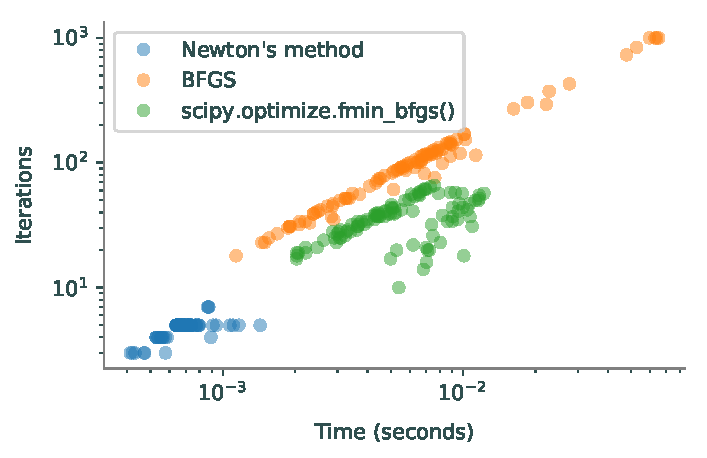
\includegraphics[width=.7\textwidth]{figures/newton_comparison.pdf}
\end{figure}
\end{problem}

\section*{The Gauss-Newton Method} % ==========================================

\subsection*{Non-linear Least Squares Problems}

Least Squares problems aim to fit a line (or model parameters) to a given set of data points.
These problems arise in many scientific fields, including economics, physics, and statistics and represent unconstrained optimization problems that minimize an objective function of the form
$$
f(\x) = \frac{1}{2}\displaystyle\sum_{j=1}^m r_j^2(\x),
$$
where each $r_i : \mathbb{R}^n \rightarrow \mathbb{R}$ is smooth and $m \geq n$.
This case of least squares problems can be solved with a Newton-like method.

Specifically, with data points $(t_1, y_1), (t_2, y_2), \ldots, (t_m, y_m)$, where $t_i,y_i \in \mathbb{R}$ for $i = 1, \ldots, m$.
Let $\phi(\x, \mathbf{t)}$ be a possible model for this data set, where $\x$ is a vector of parameters of the model, and $\mathbf{t} \in \mathbb{R}^n$.
The error at the $i$-th data point, called the \emph{residual}, is the value $$r_i(\x) := \phi(x_i, t_i) - y_i.$$
Summing the squares of these errors gives the following non-linear least squares objective function.
$$
f(\x) = \frac{1}{2} \displaystyle \sum_{j=1}^m  r_j^2(\x).
$$
The first and second derivatives of this function can then be expressed as
\begin{align*}
Df(\x) &= J(\x)\trp  r(\x), \\
D^2 f(\x) &= J(\x)\trp J(\x) + \displaystyle \sum_{j=1}^m r_j(\x) D^2r_j(\x).
\end{align*}
with $\mathbf{r}(\x) = [r_1(\x), r_2(\x), \ldots, r_m(\x)]\trp $ and
\[
J(\x) =
\left[\begin{array}{c}
\arrayrulecolor{lightgray}
D r_1(\x) \\\hline D r_2(\x) \\\hline \vdots \\\hline D r_m(\x)
\end{array}\right] \in \mathbb{R}^{m\times n}.
\]

The second term in the formula for $D^2 f$ involves second derivatives and can be problematic to compute.
In practice, the second term in the formula for $D^2 f$ is small, either because the residuals themselves are small, or because they are nearly affine in a neighborhood of the solution.
The simplest method for solving the nonlinear least squares problem, known as the \emph{Gauss-Newton Method}, exploits this observation, simply ignoring the second term and making the approximation
$$
D^2 f(\x) \approx J(\x)\trp J(\x).
$$
The method then proceeds in a manner similar to Newton's method.
Thus, at each iteration, we find $\x_{k+1}$ as follows:
\begin{equation} \label{Eq:GaussNewtonUpdate}
\x_{k+1} = \x_k-(J(\x_k)\trp J(\x_k))^{-1}J( \x_k)\trp  \mathbf{r}( \x_k).
\end{equation}

As an example, suppose we have data points generated from the function $y = 3\sin(x/2)$ and slightly perturbed by Gaussian noise.
To fit the data to a model $\phi(\x, t_i) = \phi(x_0, x_1, t_i) = x_0 \sin(x_1 t_i)$, we must select values for $\x = [x_0, x_1]\trp$ (since we know how the data was generated, we expect to find that $x_0 \approx 3$ and $x_1 \approx 1/2$).
Begin by writing functions for the proposed model, the residual vector, and the Jacobian of the residuals.

\begin{lstlisting}
>>> import numpy as np
>>> from matplotlib import pyplot as plt

# Generate random data for t = 0, 1, ..., 10.
>>> T = np.arange(10)
>>> y = 3*np.sin(0.5*T)+ 0.5*np.random.randn(10)    # Perturbed data.

# Define the model function and the residual (based on the data).
>>> model = lambda x, t: x[0]*np.sin(x[1]*t)        # phi(x,t)
>>> residual = lambda x: model(x, T) - y            # r(x) = phi(x,t) - y

# Define the Jacobian of the residual function, computed by hand.
>>> jac = lambda x: np.column_stack((np.sin(x[1]*t), x[0]*t*np.cos(x[1]*t)))
\end{lstlisting}

By inspecting the data, an initial guess for the parameters could be $x_0 = (2.5, 0.6)$.
A function implementing Gauss Newton can then be used to find the least squares solution.

\begin{lstlisting}
>>> x0 = np.array([2.5,.6])
>>> x, conv, niters = gauss_newton(jac, residual, x0, tol=1e-3, maxiter=10)

# Plot the fitted model with the observed data and the data-generating curve.
>>> dom = np.linspace(0, 10, 200)
>>> plt.plot(T, y, '*')                         # Observed data.
>>> plt.plot(dom, 3*np.sin(.5*dom), '--')       # Data-generating curve.
>>> plt.plot(dom, model(x, dom))                # Fitted model.
>>> plt.show()
\end{lstlisting}

\begin{problem} % Gauss Newton for nonlinear least squares.
Write a function that accepts a function for the proposed model $\phi(\x)$, the model derivative $D\phi(\x)$, a function that returns the residual vector $r(\x)$, a callable function that returns the Jacobian of the residual $Dr(\x) = J(\x)$, a starting point $\x_0$, a stopping tolerance \li{tol} defaulting to $1e^{-5}$, and a max number of iterations \li{maxiter} defaulting to $10$.
This method should implement the Gauss-Newton Method and return a list containing: the minimizing x value, the number of iterations performed, and if the method converged as a boolean.

Test your function by using the Jacobian function, residual function, and starting point given in the example above.
Compare your results to \li{scipy.optimize.leastsq()}.
\begin{lstlisting}
>>> minx = opt.leastsq(func=residual, x0=np.array([2.5,.6]), Dfun=jac)
\end{lstlisting}
\end{problem}

% Non-linear least squares problems can be used to analyze trends in data or to predict future events and are ubiquitous in many academic fields as well as in industrial applications and machine learning.

\begin{problem}
The file \texttt{population.npy} contains census data from the United States every ten years since 1790 for 16 decades.
The first column ($\mathbf{t}$) gives the number of decades since 1790 in the decade ($0,1,\ldots$) and the second column ($\y$) gives the population count in millions of people.

By plotting the data, and with a little knowledge about population growth, it is reasonable to hypothesize an \emph{exponential model} for the population:
\[
\phi(x_1,x_2,x_3,t) = x_1\exp(x_2(t+x_3)).
\]
Use the initial guess $(1.5, .4, 2.5)$ for the parameters $(x_1, x_2, x_3)$ and your Gauss Newton function or \li{scipy.optimize.leastsq()} to fit this model.
Plot the resulting curve along with the actual data points.

Unfortunately, the exponential model isn't a very good fit for the data because the population grows exponentially for only the first 8 or so decades.\footnote{Fitting an exponential model to only the first 8 data points results in a good model for those points (but not for later data).}
Instead, consider the following \emph{logistic model}.
$$
\phi(x_1,x_2,x_3,t) = \frac{x_1}{1+\exp(-x_2(t+x_3))}.
$$
A reasonable initial guess for the parameters $(x_1, x_2, x_3)$ is $(150, .4, -15)$.
Write functions for the model and the corresponding residual vector, then fit the model.
Plot the data against the fitted curve (in the same plot as before).
It should be a much better fit than the exponential curve.
\end{problem}

\begin{comment}

%%% OLD GAUSS NEWTON
The individual functions $r_i$ that measure the error between the model and the data point are known as \emph{residuals},
and we can aggregate these functions into a \emph{residual vector}
$$
\mathbf{r}(\x) := (r_1(\x), r_2(\x), \ldots, r_m(\x))\trp .
$$
The Jacobian of $\mathbf{r}(\x)$ can be expressed in terms of the gradients of each $r_i$ as follows:
%% TODO: put this back in!
$$
J(\x) = \begin{bmatrix} D r_1(\x)\trp  \\ D r_2(\x)\trp  \\ \vdots \\ D r_m(\x)\trp  \end{bmatrix}
$$
You can further verify that
\begin{align*}
D f(\x) &= J(\x)\trp  r(\x), \\
D^2 f(\x) &= J(\x)\trp J(\x) + \displaystyle \sum_{j=1}^m r_j(\x) D^2r_j(\x).
\end{align*}

In particular, at the $k$-th iteration, we choose a search direction $p_k$ that solves the linear system
$$
J_k\trp J_kp_k = -J_k\trp r_k.
$$

For convenience, we summarize these steps in Algorithm \ref{alg:guassnewton}.

\begin{algorithm}
\begin{algorithmic}[1]
\Procedure{Gauss-Newton}{}
    \State \textrm{Choose initial parameter vector } $x_0$
    \State $k \gets 0$
    \While{$J_k\trp r_k \neq 0$}
        \State \textrm{solve } $J_k\trp J_kp_k = -J_k\trp r_k$
        \State \textrm{choose step size } $\alpha_k$ \textrm{ satisfying Wolfe Conditions.}
        \State $x_{k+1} \gets x_k + \alpha_kp_k$
        \State $k \gets k+1$
    \EndWhile
\EndProcedure
\end{algorithmic}
\caption{Gauss-Newton Method}
\label{alg:guassnewton}
\end{algorithm}

Now we write Python functions for our model, the residual vector, the Jacobian, the objective function,
and the gradient. The calculations for all of these are straight forward.
\begin{lstlisting}
>>> def model(x, t):
>>>     return x[0]*np.sin(x[1]*t)
>>> def residual(x):
>>>     return model(x, t) - y
>>> def jac(x):
>>>     ans = np.empty((10,2))
>>>     ans[:,0] = np.sin(x[1]*t)
>>>     ans[:,1] = x[0]*t*np.cos(x[1]*t)
>>>     return ans
>>> def objective(x):
>>>     return .5*(residual(x)**2).sum()
>>> def grad(x):
>>>     return jac(x).T.dot(residual(x))
\end{lstlisting}
By inspecting our data, we might make an initial guess for the parameters $x_0 = (2.5, 0.6)$.
We are now ready to use our \li{gaussNewton} function to find the least squares solution.
\begin{lstlisting}
>>> x0 = np.array([2.5,.6])
>>> x = gaussNewton(jac, residual, x0, niter=10)
\end{lstlisting}
We can plot everything together to compare our fitted model with the data and the original sine
curve from which the data were generated.
\begin{lstlisting}
dom = np.linspace(0,10,100)
plt.plot(t, y, '*')
plt.plot(dom, 3*np.sin(.5*dom), '--')
plt.plot(dom, x[0]*np.sin(x[1]*dom))
plt.show()
\end{lstlisting}


The module \li{scipy.optimize} also has a method to solve non-linear least squares problem, and it is quite convenient.
The function is called \li{leastsq()}, and in its most basic use, you only need
to pass in the residual function and starting point as arguments.
In the example above, we simply need to execute the following code:
\begin{lstlisting}
>>> from scipy.optimize import leastsq
>>> x2 = leastsq(residual, x0)[0]
\end{lstlisting}
This should give us the same answer, but much faster.

%% TODO: put this back in!
Thus, your new model is
$$
\phi(x_1,x_2,x_3,t) = \frac{x_1}{1+\exp(-x_2(t+x_3))}.
$$
By inspection, find a reasonable
initial guess for the parameters $(x_1, x_2, x_3)$ (i.e. $(150, .4, -15)$).
Again, write Python functions for the model and the corresponding residual vector,
and fit the model. Plot the data against the fitted curve. It should be a good fit.
\end{comment}
